\section{Experimental Evaluation}\label{sec:evaluation}

We performed three different sets of experiments, using four domains that materialize the continuum. The first set was devised to \emph{study how latency changes with a varying workload}. In this case the mobile domain is obviously omitted. The second set was devised to \emph{evaluate the domains from the perspective of the client}, both in terms of latency and battery consumption. The third set was devised to \emph{evaluate the A3-E approach with domains that change their availability} according to a probabilistic model. 
%Our goal was to demonstrate that the A3-E model is successful in selecting domains at run time and in improving the overall application availability. 

\subsection{Domains Setup}

%\subsubsection{Domains}

We deployed a set of domains that materialize the computing continuum --- as shown in Table~\ref{tab:domain-exp-config}. The sample application is an Image Recognition one, in which users can capture an image and invoke microservices~\footnote{Microservice implementation available in \url{https://github.com/deib-polimi/A3-E-image-recognition}} in the continuum to perform the \textit{extraction of features} and \textit{detection of objects} in the image. For our mobile domain we used a smartphone in which we deployed the A3-E middleware and the functions needed to perform both feature extraction and object identification. For our local-edge domains we adopted the Apache OpenWhisk serverless platform, as the state-of-the-art open-source solution. We had two local-edge domains, and placed both of them in the same LAN as the origin of the requests (i.e., the client applications/devices). This was done to emulate a few-hops scenario in which devices are directly connected to their nearest edge domains. \texttt{Local-edge-1} allows us to represent a situation in which latency is close to zero, but the computational resources are highly constrained, as scaling-up is not possible due to the inherent physical restrictions of the underlying infrastructure. \texttt{Local-edge-2} has more computational resources and yet low latency can be achieved due to physical proximity.

\begin{table}[htb]
	\caption{Domains Setup in the Continuum for the Experimental Evaluation}
	\label{tab:domain-exp-config}
	\small
	\begin{tabular*}{1\textwidth}{@{\extracolsep{\fill}}>{\raggedright}p{1.7cm}>{\raggedright}p{6cm}>{\raggedright}p{5cm}}
		\toprule 
		Domain & Machine Resources & Execution Environment\tabularnewline
		\midrule
		\midrule 
		Mobile & Samsung Galaxy S6 SM-G90, 3Gb RAM, 8x Cortex CPU 2Ghz & Android 5.0.2 + Java Functions + OpenCV
		\tabularnewline
		\midrule 
		Local-edge-1  & ubuntu/trusty64-2, 4x vCPUs, 4Gb RAM & OpenWhisk, 256 Mb/Action, Python 2.7 + OpenCV \tabularnewline
		\midrule 
		Local-edge-2  & ubuntu/trusty64-2, 8x vCPUs, 16Gb RAM & OpenWhisk, 256 Mb/Action, Python 2.7 + OpenCV \tabularnewline
		\midrule 
		Cloud-FaaS & N/A & AWS Lambda, 256 Mb/Function, Python 2.7 + OpenCV \tabularnewline
		\midrule 
		Cloud-IaaS & Auto Scaling Group with t2.micro instances + Amazon Linux AMI 2017  & NodeJs 6.11 server + Python 2.7 + OpenCv
		\tabularnewline
		\bottomrule
	\end{tabular*}
\end{table}


%In this experiment, we considered two alternatives for deploying the serverless continuum architecture, mimicking the behavior of both an edge node and a fog node (Figure~\ref{fig:exp-edge}).  

%The client application is embedded in the edge node, consisting on the postman requests and the node.js endpoint (Figure~\ref{fig:exp-setup1}). 
%On the edge-local alternative, we used a virtual machine running locally, on a regular laptop, with 4x CPU, 4x Gb of RAM and 40 Gb SSD of storage. 

%For the Fog alternative, we deployed the serverless architecture on Policloud\footnote{http://policloud.polimi.it/}, the private IaaS solution of Politecnico di Milano. Here, the computational resources are less constrained, and still low latency can be achieved due to physical proximity (two hops from the client) and data locality. This setup runs on a small cluster of 4 virtual machines with 2x CPU, 4x Gb of Ram and 100 GB SSD, each running a different component of openwhisk (triggers and storage, Http server, controller, and invokers, respectively). Note that in this case the fog node is deployed in the same LAN that originates the requests, to emulate the few-hop scenario in which devices are directly connected to their corresponding MEC.

The cloud domain for this experiment used AWS Lambda, as the most mature serverless solution on the market. The functions and associated libraries and dependencies (storage, feature extraction and matching) were hosted within the same AWS region. This is actually enforced by AWS to guarantee a certain degree of data locality. Finally, we also deployed the functionality onto a traditional cloud domain, i.e., using cloud IaaS. 

The main goal of this setup was not to compare traditional cloud services against a serverless solution, but to demonstrate that the proposed continuum could outperform the cloud under the tested circumstances and requirements.



\subsection{Domain Latency} 


%\begin{figure}[htb]
%	\centering
%	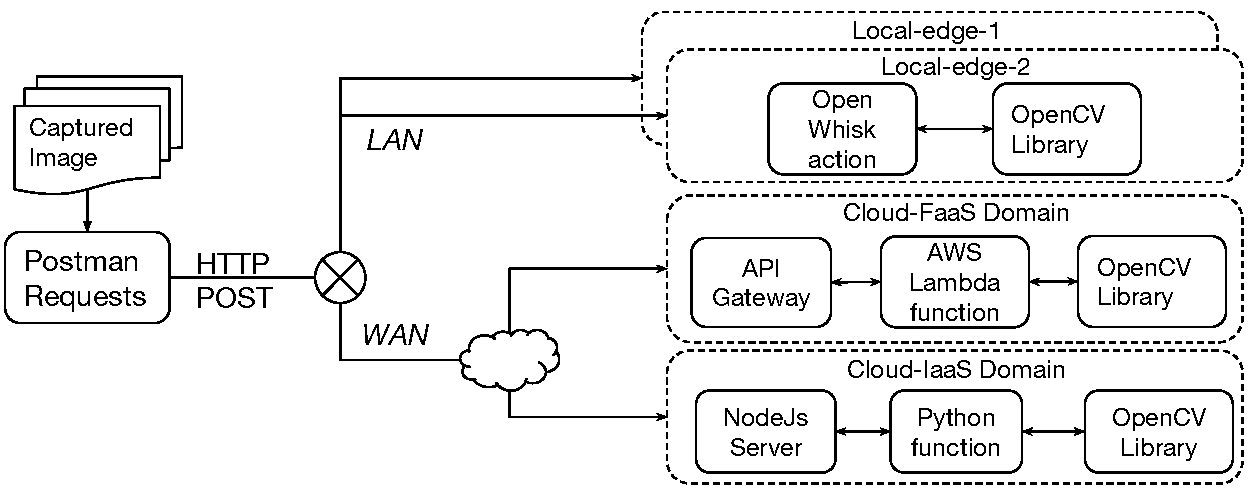
\includegraphics[width=0.95\textwidth]{figs/experimental-setup.pdf}
%	\caption{Setup for Domain Latency Experiments}
%	\label{fig:exp-setup1}
%\end{figure}

The first experiment assesses how the latency changes with a varying workload, as a baseline to compare different domains. We simulated different number of clients making $100$ requests each, at a constant rate of two requests per second. Each request stimulated both the feature extraction and the matching from a sample image. This setup was achieved taking into account the default maximum for concurrent executions in AWS Lambda\footnote{\url{http://docs.aws.amazon.com/lambda/latest/dg/concurrent-executions.html}} and Openwhisk\footnote{\url{https://github.com/apache/incubator-openwhisk/blob/master/docs/reference.md}}, as well as the limited resources of the edge domains. 

This experiment excluded the mobile domain and focused on the remote ones, i.e., edge and cloud. Capturing and uploading an image was emulated using Postman\footnote{\url{https://www.getpostman.com/}}, an open source application designed to load test the functional behaviors of Web APIs, and to measure their performances. The payload for this experiment was a sample image of approximately 65 KB, which is a reasonable size for this use case considering the requirements regarding low-latency and computation time~\cite{rodriguez16mobile}. 

%Once the image was sent through HTTP/POST, the actual execution depended on the domain being used. triggering Openwhisk actions for both edge domains, AWS Lambda functions for Cloud-FaaS domain, and a Nodejs server that calls a Python function for Cloud-IaaS domain.

%was performed without using the A3-E middleware nor the device (mobile domain), since it aims to evaluate the plain latency for remote domains when processing simultaneous requests. This scenario would not occur in a mobile domain, which only process local requests. The possibility of offloading computation from one mobile device to another is left as a future work.



 

%In our edge domains for the experiment, uploading an image to CouchDB (Step 3.a) triggers the action that performs the feature extraction and matching (Step 4.a)  with the points-of-interest, supported by the OpenCV\footnote{\url{http://opencv.org}} visual recognition library (Step 5.a). 




%\subsubsection{Baseline Latency}

 Figure~\ref{fig:latency-domains} shows the average latency for each scenario, averaged through $5$ executions. Note that the computation time (light gray) is different from the overhead (dark gray). The latter includes network communication (routing and forwarding) and queuing time (when no resources are available to process the request immediately). 

\begin{figure}
	
	\centering
	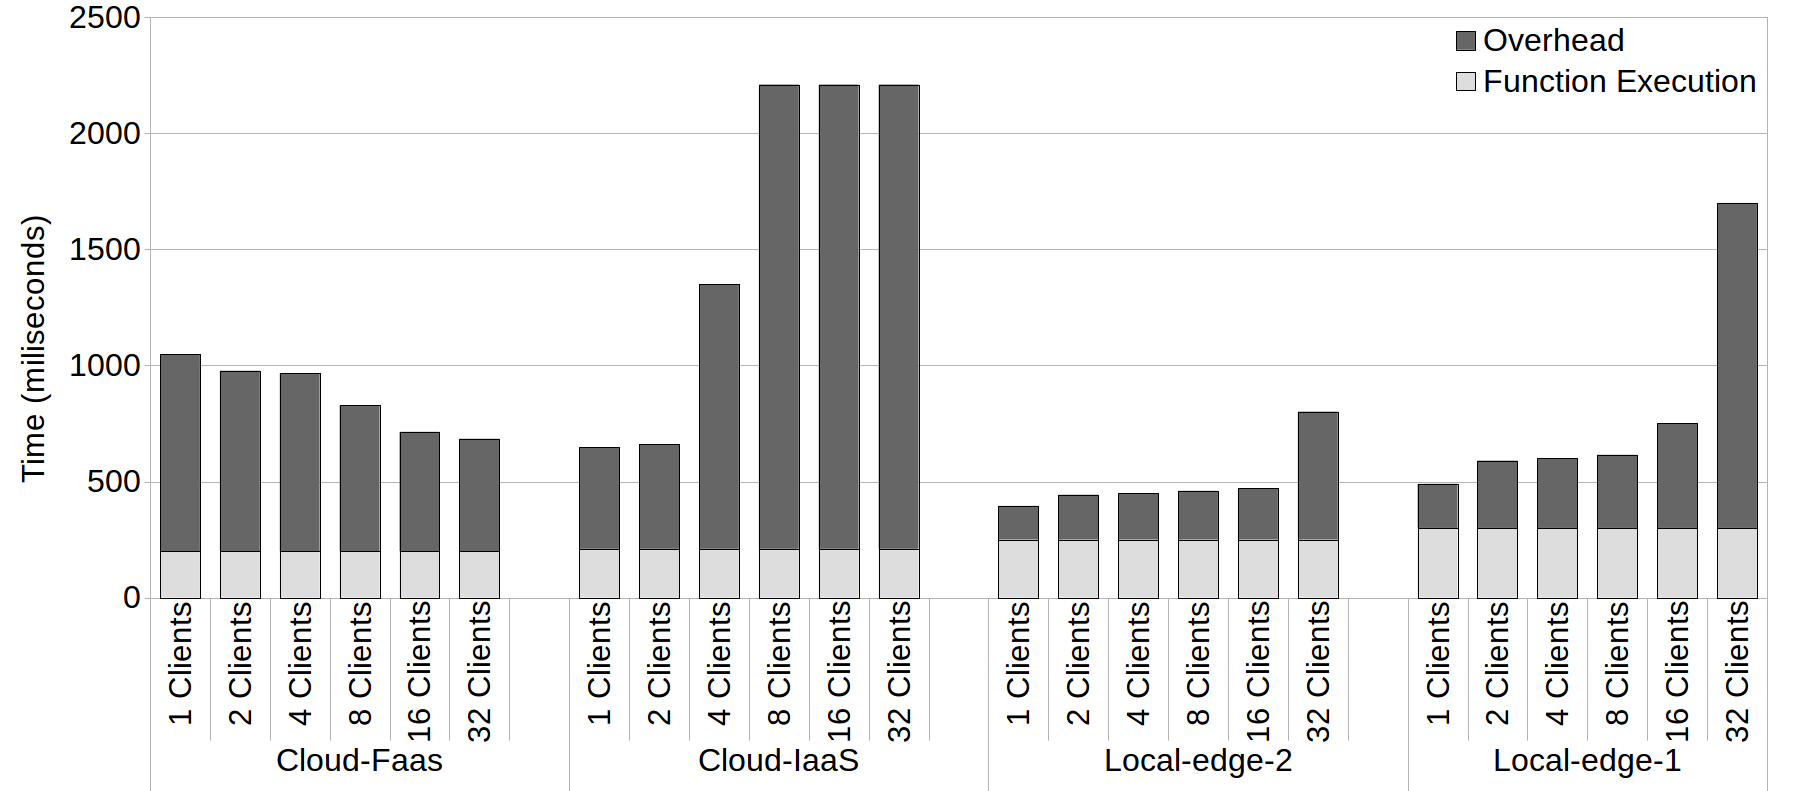
\includegraphics[width=1\textwidth]{figs/latency-domains}
	\caption{Latency results for each domain and different number of clients.}
	\label{fig:latency-domains}
\end{figure}

 When considering up to $16$ simultaneous clients, the latencies added by the edge domains are less than the latencies in both cloud alternatives. Regarding the \textit{cloud-FaaS} domain, the latency reduction is up to $90$\% for \texttt{local-edge-1} and up to $82$\% for \texttt{local-edge-2} respectively. Regarding the \textit{cloud-IaaS} domain, reductions are up to $77$\% and $58$\%, respectively. Since in \textit{cloud-IaaS} a scaling-up action (that can demand several seconds~\cite{Quatrocchi2016discrete}) triggers when more than one VM instance is needed to handle the workload, requests timeout in the meantime. 
 
 For light to medium workloads, the local-edge domains outperformed all the other alternatives. However, \texttt{local-edge-1} is the most resource-constrained, which hinders its availability under heavier workloads. Interestingly, \textit{cloud-IaaS} also outperformed  \textit{cloud-FaaS} ($46$\% less latency) for light workloads. This can be due to the additional steps performed by the API Gateway in order to forward RESTful calls to AWS lambda functions in  \textit{cloud-FaaS}\footnote{http://docs.aws.amazon.com/lambda/latest/dg/with-on-demand-https.html}. Nevertheless, this advantage is mitigated by the fact that \textit{cloud-FaaS} can better react to workload bursts, thanks to its faster horizontal scaling~\cite{Villamizar2017lambda,Hendrickson:2016}.


%\subsection{Battery} The second set of experiments targeted the measurement of battery consumption of a mobile device in two scenarios: 1) in which feature extraction and matching were performed locally, and 2) these tasks were offloaded to edge servers.

\subsection{A3-E in the Continuum} 

In our second set of experiments the main goal is to evaluate the continuum from the client's perspective, in terms of battery consumption and latency. A mobile device was setup to host the A3-E middleware, which was in charge of  selecting the best domain for a specific execution, based on the perceived QoS. 
Once again our sample application was the image recognition one with feature extraction and matching provided along the continuum. In this case we had three domains: \textit{mobile}, \textit{local-edge} and \textit{cloud-FaaS} (see Table~\ref{tab:domain-exp-config}). The experiment featured four different scenarios: the first three consider one domain each, and the last one (\textit{all-domains}) combines the previous ones to form the continuum. Details on how we modeled the availability of each domain in the \textit{all-domains} scenario are discussed in Section~\ref{sub:domain-selection}.

\begin{comment}
internetOnToOffProbability = 0.22%
internetOffToOnProbability = 1.66%

edgeOnToOffProbability = 3.33%;
edgeOffToOnProbability = 6.66%;

e = 1/p; //average number of trials it takes for the event with probability p to happen
~t = e * u;  //average time it takes for the event with probability p to happen given a trial interval u
~t = u/p; //the same, but using the trial interval and the probability p 

###

trial interval u = 2 seconds

average time for disconnecting: 15 x 60 seconds
prob. of disconnecting: 0.2222222%   

average time for reconnecting: 2 x 60 seconds
prob. of reconnecting: 1.666666%

average time for edge unavailability: 10 x 60 seconds 
prob. of edge unavailability: 0.333333%

average time for edge becoming available: 5 x 60 seconds 
prob. of edge becoming available: 0.666666%

\end{comment}

%(all-domains).

The experiment consisted in cascading $2000$ sequential requests for feature extraction and matching of a sample image (with a size of 65 KB). We measured the total execution time, the battery consumption in the mobile device, and the average time per call. Figure~\ref{fig:exp-a3e} shows the experimental results, averaged among $5$ executions for each scenario.

\begin{figure}[htb]
	\centering
		\captionsetup[subfigure]{width=0.45\textwidth}	
	\subfloat[Total execution time (seconds)\label{fig:total-exec-a3e}] {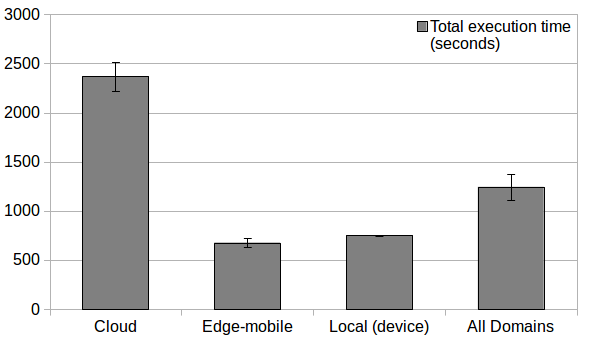
\includegraphics[width=0.45\textwidth]{figs/total-exec-time-A3E}}	\captionsetup[subfigure]{width=0.45\textwidth}
	\subfloat[Battery consumption (\%)\label{fig:battery-a3e}] {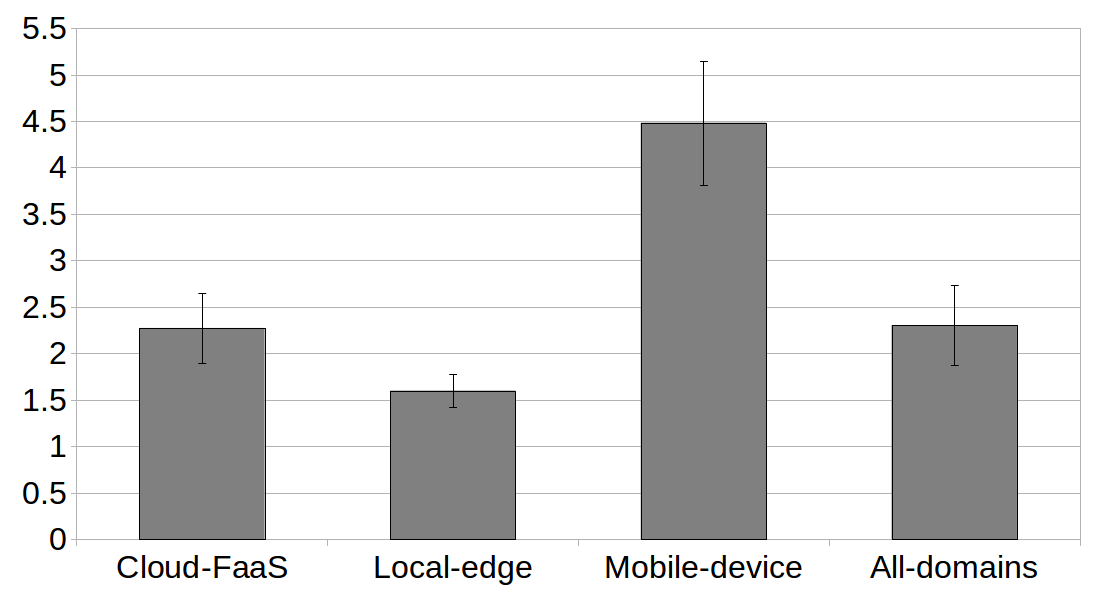
\includegraphics[width=0.45\textwidth]{figs/battery-consumption-A3E}}
	
	\centering
	
	\captionsetup[subfigure]{width=0.45\textwidth}	\subfloat[Execution time per call (ms)\label{fig:time-per-call-a3e}] {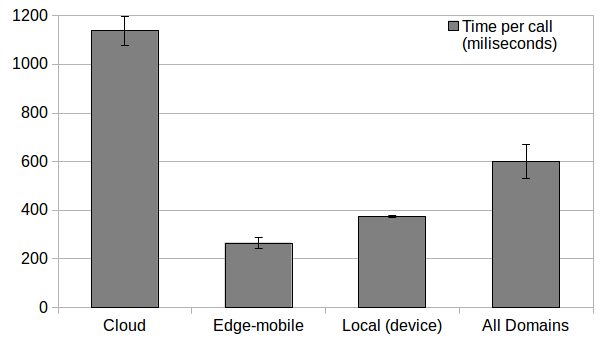
\includegraphics[width=0.45\textwidth]{figs/time-per-call-A3E}}
	%\captionsetup[subfigure]{width=0.45\textwidth}
	%\subfloat[Number of Calls per domain in all-domains scenario\label{fig:calls-per-domain-a3e}] {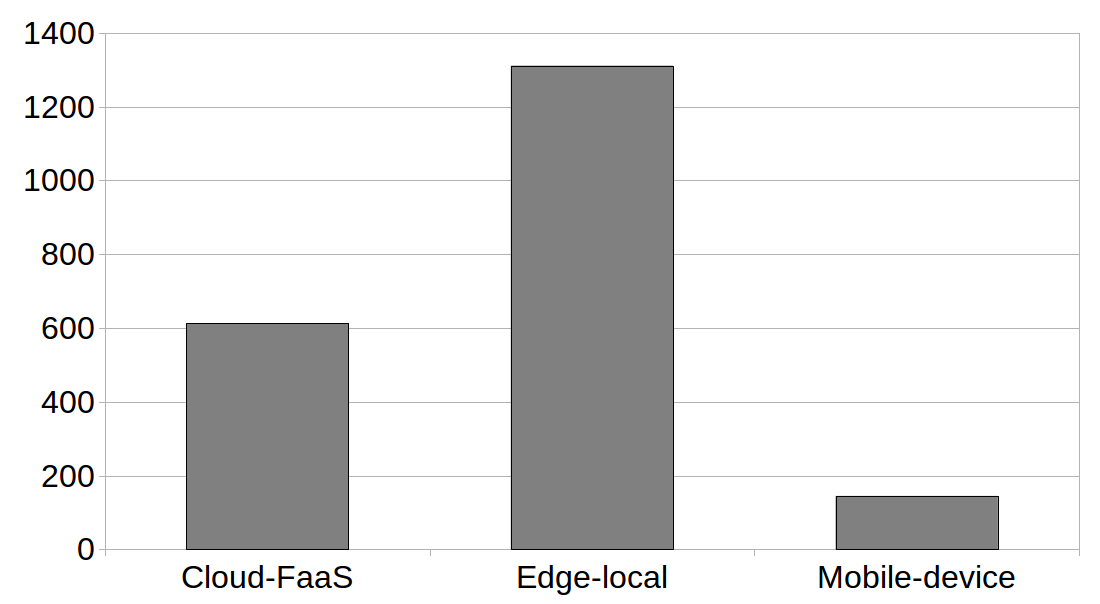
\includegraphics[width=0.45\textwidth]{figs/calls-per-domain-A3E}}	
	\caption{A3-E experimental evaluation results} \label{fig:exp-a3e}
\end{figure}

%\begin{figure}[htb]
	%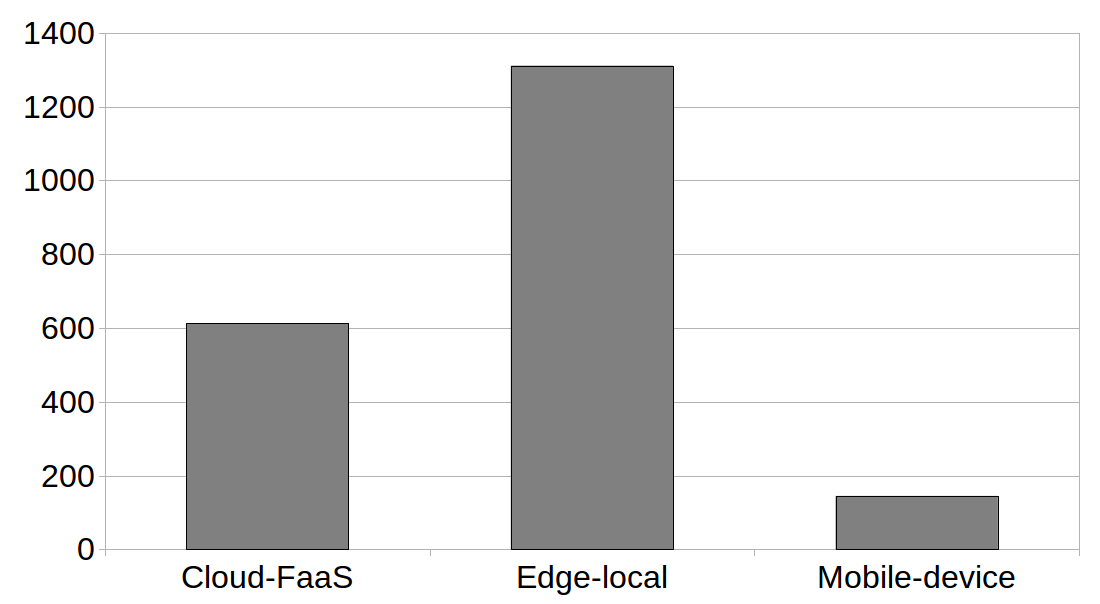
\includegraphics[width=0.45\textwidth]{figs/calls-per-domain-A3E}
	%\caption{Number of Calls per domain in all-domains scenario}
	%\label{fig:calls-per-domain-a3e}
%\end{figure}

For the total execution time (Figure~\ref{fig:total-exec-a3e}), considering the \texttt{Cloud-FaaS} domain as a baseline, \texttt{local-edge} improved the execution time up to a $72$\%, while \texttt{mobile} and \texttt{all-domains} up to a $69$\% and $49$\%, respectively. The highest battery consumption (see Figure~\ref{fig:battery-a3e}) was when using only the \texttt{mobile} domain, with a battery drop of $4.5$\% during $750$ seconds (i.e., $12.5$ minutes) of execution. Battery savings with \texttt{Cloud-FaaS}, \texttt{local-edge} and \texttt{all-domains} were $49$\%, $35$\%, and $49$\%, respectively. The average execution time (see Figure~\ref{fig:time-per-call-a3e}), with \texttt{Cloud-FaaS} as our baseline ($1137$ milliseconds per call), was improved by $76$\%, $68$\% and $47$\% for \texttt{local-edge}, \texttt{Mobile} and \texttt{all-domains}, respectively. 

These experiments tell us that the total execution time, when using only the cloud, was two times higher than when using the continuum (\texttt{all-domains}). Since the requests were performed in cascade and given the higher latency per call in the cloud, the total time increases accordingly. Clearly, using A3-E to switch to edge domains when possible substantially reduces the latency and improves the perceived QoS.

Battery consumption was substantially lower when offloading computation, rather than performing it on the device. The \texttt{mobile}-device scenario lasted half the time, but used twice as much battery (a prohibitive $20$\% of battery drain per hour) than the \texttt{all-domains} one, given that it was performing CPU intensive operations. This recalls the importance of computation offloading to preserve a device's resources.

\subsection{Dynamic Domain Selection in the Continuum}
\label{sub:domain-selection}

Finally, we evaluated the capability of the A3-E prototype to select the best domain given low latency and high computational power requirements. In this experiment we used all three domains together to form the continuum, and probabilistically simulated their availabilities. 

A3-E was configured to ping for domain availability, as well as perceived QoS, every two seconds ($u = 2$). We consider that the cloud domain could be unavailable mainly due to absence of mobile network's coverage, since downtimes of cloud services are minimal~\cite{garcia2017bandwidth}. To simulate this, the average network unavailability was set to once every $15$ minutes. Then, the average time for it to become available again was $2$ minutes, which gives us a probability \textit{connectionAvailable} $=15/(15+2)=0.88$.

%\footnote{https://math.stackexchange.com/questions/165993/average-number-of-times-it-takes-for-something-to-happen-given-a-chance}

The rationale for the edge domain is analogous, yet with a higher probability of it being unavailable --- e.g., due to the lack of physical proximity with the edge servers. In this case, the edge is unavailable once every $10$ minutes, and it would take an average of $5$ minutes for it to become available again. Therefore, the probability \textit{edgeAvailable} $=10/(10+5)=0.66$. If we consider that edge nodes are only reachable within network coverage, then the probability \textit{edgeAvailableWithConnection}$=0.88*0.66=0.58$.

Finally, we consider the mobile device as always available, and therefore it was selected in our experiments when all other domains were unavailable, or the sensed latencies were too high for the application's requirements.

%To simulate the cases in which the mobile device was momentarily outside of the mobile network's coverage, the average unavailability of the cloud domain~\cite{garcia2017bandwidth} was set to once every $15$ minutes. A3-E was configured to ping for domain availability, as well as perceived QoS, every two seconds ($u = 2$). Using a geometric distribution, the probability of the cloud being unavailable during a ping (\textit{internetOnToOff}) was $0.022$. Every time the cloud was unavailable, the average time for it to become available again was $2$ minutes, i.e., the probability  \textit{internetOffToOn} was $0.166$. Overall, this gives us a probability \textit{internetAvailability} $=15/(15+2)=0.88$.

%\footnote{https://math.stackexchange.com/questions/165993/average-number-of-times-it-takes-for-something-to-happen-given-a-chance}

%The rationale for the edge domain is analogous, yet with a higher probability of it being unavailable --- e.g., due to the lack of physical proximity with the edge servers. In this case, the edge is unavailable once every $10$ minutes, i.e., the probability was \textit{edgeOnToOff}  $ = 0.33$. Once unavailable, we considered that it would take an average of $5$ minutes for it to become available again, i.e. the probability \textit{edgeOffToOn} was $0.066$. Therefore, the probability \textit{edgeAvailability} $=10/(10+5)=0.66$. If we consider that edge nodes are only reachable within network coverage, then the probability \textit{edgeAvailabilityWithAvailable}$=0.88*0.66=0.58$.

%Finally, we consider the mobile device as always available, and therefore it was selected in our experiments when all other domains were unavailable, or the sensed latencies were too high for the application's requirements.

Figure~\ref{fig:all-domains} shows detailed results for the \texttt{all-domains} scenario with regards to availability and consistency. Given the availability probabilities for edge and cloud discussed above, the experiment shown (see Fig.~\ref{fig:availability-all-domains}) an average of $93\%$ availability without considering the \texttt{mobile} domain ($5\%$ and $35\%$ improvement regarding cloud and edge respectively), and $100\%$ availability when considering also the \texttt{mobile} domain (which is always available). 

Figure~\ref{fig:calls-per-domain-a3e} shows the average number of calls processed by each domain in the continuum: $63$\% by \texttt{local-edge}, followed by \texttt{cloud-FaaS} ($30$\%) and \texttt{mobile} ($7$\%). In terms of consistency, given that all requests were served, on average $70\%$ of the requests perceived low latency, whilst the $30\%$ that relied on the cloud perceived a degradation in the QoS but still were processed successfully. 
 
\begin{figure}[htb]
	\centering

	\captionsetup[subfigure]{width=0.45\textwidth}
	\subfloat[Average availability per domain (\%)\label{fig:availability-all-domains}] 
	{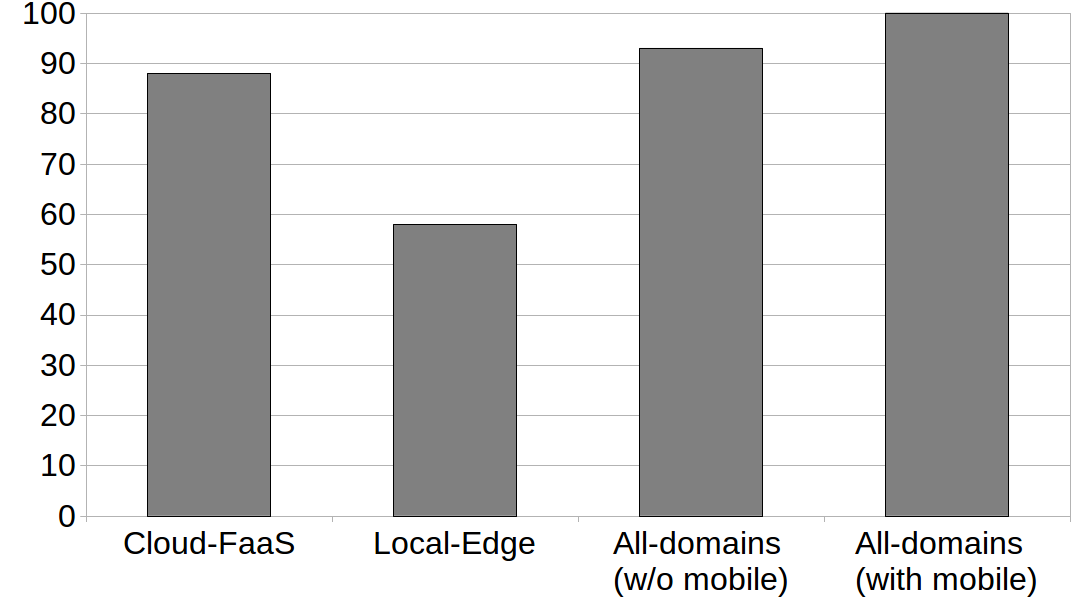
\includegraphics[width=0.45\textwidth]{figs/availability-all-domains}}
	\captionsetup[subfigure]{width=0.45\textwidth}
	\subfloat[Number of requests served per domain\label{fig:calls-per-domain-a3e}] {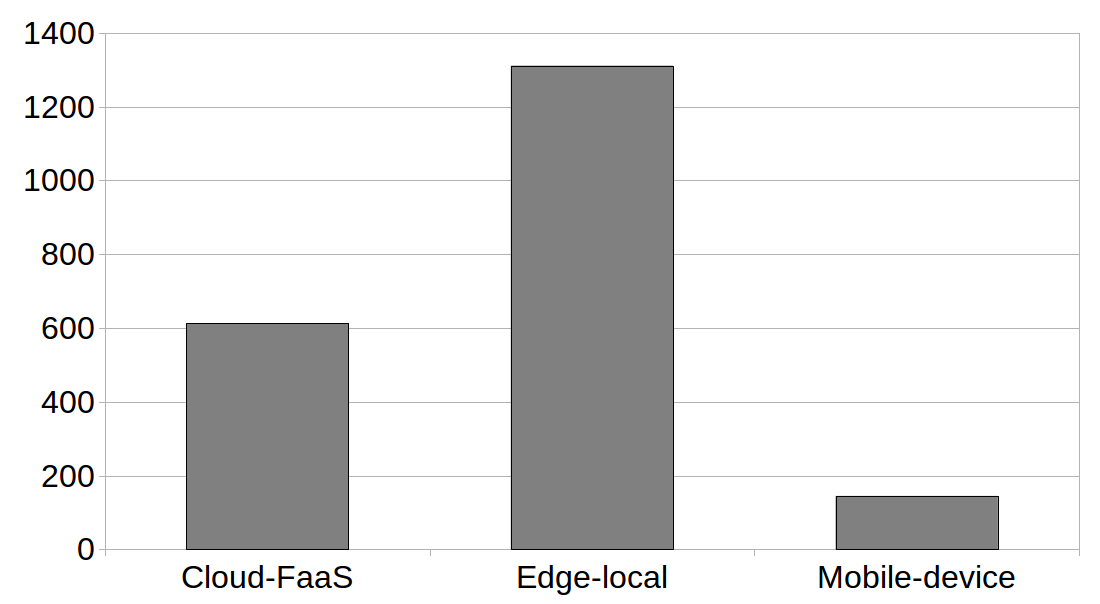
\includegraphics[width=0.45\textwidth]{figs/calls-per-domain-A3E}}
	
	\caption{All-domains scenario results} \label{fig:all-domains}
\end{figure}

Conclusively, the experiment shown that A3-E is capable of performing domain selection and computation distribution at runtime. A3-E also improved availability up to 100\% during the experiment, given that the mobile domain is always available, but it was only selected to serve 7\% of the requests.
In the context of the \texttt{all-domains} scenario, this reflects the underlying rationale of the computation continuum: exploit the edge domains as much as possible (by giving them high scores in Formula~\ref{eq:smart}). This will lead to better balance among computation time, latency and resource consumption. Switch to the cloud, or to the local device, only when necessary. Note that in this experiment computation in the mobile device was configured with the lowest possible score, thus the cloud was selected as the first alternative to edge domains. This behavior can be tuned by adjusting application requirements and domain parameters discussed in Section~\ref{sec:implementation}.

%that allows to cope with unavailability and fluctuations in QoS 

%\textcolor{blue}{TODO:(2) Discuss the relevance of the results }

%\paragraph{Threats to validity}

In terms of threats to validity is it worth mentioning that the experiments only targeted one client application (image recognition) and, in the case of the second experiment, only one client device. Further tests are needed, considering multiple clients using several applications with different requirements (in addition to latency and computational power) and their corresponding functions deployed along the continuum. Additionally, it is currently not possible to test with real mobile-edge domains, i.e., to provide computational capabilities on base stations. This could be approximated either by simulation or by deploying edge domains following current specifications of \textit{mobile edge computing} in terms of computational power and latency to better capture the heterogeneity of the continuum. Nonetheless, the fact that specifications and technologies are still being worked/researched limits the accuracy in which mobile-edge domains can be evaluated.  %Finally, even though the all-domains scenario provided insights regarding availability and consistency, experiments focusing particularly on consistency, correctness and reliability of the model are outside the scope of the paper and thus left as future work.



